\chapter{Classical Mechanics Review}
\section{Introduction to Classical Systems}

In classical mechanics, the fundamental task is to describe the state and the evolution of a physical system composed of a certain number of particles. Each particle is uniquely characterized by its position and momentum, which together form a set of canonical conjugate variables. For \(N\) identical particles moving in a space of dimension \(d\), the state of the \(i\)-th particle is represented by the pair:
\[
  (q_i, p_i) \in M,
\]
where \(M\) denotes the \textbf{phase space}, a \(2d\)-dimensional manifold that encompasses all possible positions and momenta. The total state of the system, or its \textit{microscopic state}, is then given by the collection of all the particle states:
\[
  \{(q_i, p_i)_{i=1}^{N}\} \in M^N.
\]

An \textbf{observable} is any physical quantity that can be assigned a numerical value once the state of the system is specified. Mathematically, an observable is represented by a smooth real function defined on the phase space:
\[
  f : M^N \to \mathbb{R}.
\]
The \textbf{measurement} of such an observable in a particular state corresponds simply to evaluating the function at the point representing that state:
\[
  f(\overline{q}_i, \overline{p}_i).
\]
Typical examples of observables include the total energy, the angular momentum, or the center-of-mass position of the system.

\subsection*{Dynamics and Hamilton's Equations}

The time evolution of the system is not arbitrary: it is determined by a distinguished observable, the \textit{Hamiltonian function} \( H(q_i, p_i; t) \), which typically represents the total energy of the system. According to Hamilton's formulation of mechanics, the equations of motion are given by the system of first-order differential equations:
\[
  \dot{q}_i = \frac{\partial H}{\partial p_i}, \qquad \dot{p}_i = -\frac{\partial H}{\partial q_i}.
\]

These equations describe how positions and momenta vary in time under the action of the Hamiltonian flow.

\paragraph{Conservation of energy.} If the Hamiltonian does not depend explicitly on time, the system is said to be \textit{autonomous}, and the total energy is conserved along the trajectories:
\[
  E \equiv H(q_i(t), p_i(t)) = H(q_i(0), p_i(0)).
\]

\paragraph{Liouville's theorem.} A fundamental geometric property of Hamiltonian systems is that their flow in phase space preserves the natural volume element, a result known as \textit{Liouville's theorem}. This means that although the system evolves and individual trajectories may become highly complex, the total volume in phase space occupied by a collection of states remains invariant over time. This property underpins many results in statistical mechanics, where ensembles of states are studied rather than single trajectories.

\begin{figure}[H]
  \begin{minipage}{0.5\textwidth}
    \centering
    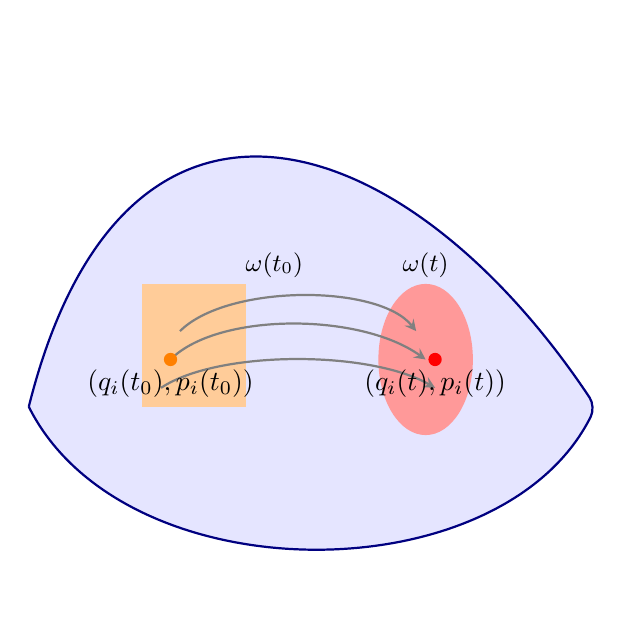
\begin{tikzpicture}[scale=1.2, >=stealth]

      \fill[blue!10,rounded corners] (0,0) .. controls (1,4) and (4,3) .. (6 ,0)
      .. controls (5,-2) and (1,-2) .. (0,0);
      \draw[blue!50!black,thick,rounded corners] (0,0) .. controls (1,4) and (4,3) .. (6,0)
      .. controls (5,-2) and (1,-2) .. (0,0);

      \fill[orange!40] (1.2,0.0) rectangle (2.3,1.3);
      \node at (2.6,1.5) {\small \(\omega(t_0)\)};

      \fill[red!40] (4.2,0.5) ellipse (0.5 and 0.8);
      \node at (4.2,1.5) {\small \(\omega(t)\)};

      \draw[->,thick,gray] (1.5,0.5) .. controls (2.0,1.0) and (3.5,1.0) .. (4.2,0.5);
      \draw[->,thick,gray] (1.4,0.2) .. controls (2.0,0.6) and (3.6,0.6) .. (4.3,0.2);
      \draw[->,thick,gray] (1.6,0.8) .. controls (2.1,1.3) and (3.7,1.3) .. (4.1,0.8);

      \fill[orange] (1.5,0.5) circle (2pt) node[black,below] {$(q_i(t_0), p_i(t_0))$};
      \fill[red] (4.3,0.5) circle (2pt) node[black,below] {$(q_i(t), p_i(t))$};
    \end{tikzpicture}
  \end{minipage}
  \hfill
  \begin{minipage}{0.48\textwidth}
    Initial condition \((q_i(t_0), p_i(t_0))\) evolves to \((q_i(t), p_i(t))\) under Hamiltonian flow. The volume of any region \(\omega(t_0)\) in phase space is preserved over time, i.e., \(\text{Vol}(\omega(t_0)) = \text{Vol}(\omega(t))\). Consequently, the density of states in phase space remains constant along the trajectories, which implies the conservation of the total number of states.
  \end{minipage}
\end{figure}

\section{Statistical Description}

Hamilton's equations are deterministic: once the initial conditions \(q_i(t_0), p_i(t_0)\) are specified, the system of first-order differential equations admits a unique solution \( (q_i(t), p_i(t)) \) for all times, provided the Hamiltonian is sufficiently smooth. Thus, the evolution in phase space is uniquely determined and reversible, as the flow defines a one-to-one mapping between initial and final states. Each such trajectory corresponds to a \textbf{microstate} of the system, fully characterizing its dynamical evolution.

However, in many practical situations the exact specification of the initial conditions is either impossible or irrelevant. What we can measure in experiments are not the detailed positions and momenta of all particles, but rather macroscopic quantities such as energy, volume, pressure, or particle number. Different microscopic configurations \((q_i(t),p_i(t))\) may correspond to the same values of these thermodynamic variables, and are therefore indistinguishable from a physical point of view. This motivates the introduction of a \textbf{macrostate}, which is defined not by a single trajectory in phase space, but by a whole set of microstates compatible with the observed macroscopic conditions.

To analyze such systems, statistical mechanics introduces the concept of an \textbf{ensemble}: a large collection of virtual copies of the system, each representing a possible microstate consistent with the given macrostate. The ensemble provides a probabilistic description of the system, allowing us to replace detailed knowledge of microscopic trajectories with statistical averages over all accessible states. In this framework, thermodynamic quantities emerge naturally as expectation values of the corresponding observables.

\subsection*{Probability Distributions in Phase Space}

For a large ensemble, the microscopic uncertainty about the state of the system is encoded in a probability density function
\[
  \rho(q_i, p_i; t)
\]
defined on the phase space \(\mathcal{M}\). This function satisfies the standard properties of a probability distribution, i.e. \textit{positivity} and \textit{normalization}:
\[
  \rho(q_i, p_i; t) \geq 0,
  \qquad
  \int_{\mathcal{M}} \rho(q_i, p_i; t) \prod_i dq_i \, dp_i = 1,
\]
so that the total probability of finding the system somewhere in phase space is normalized to unity.

The probability of finding the system in a particular subset
\(\mathcal{U} \subset \mathcal{M}^N\) is then obtained by integrating the density over that region:
\[
  \mathbb{P}[(q_i, p_i) \in \mathcal{U}]
  = \int_{\mathcal{U}} \rho(q_i, p_i; t) \prod_i dq_i \, dp_i.
\]

Since the phase-space measure \(\prod_i dq_i \, dp_i\) carries physical dimensions, it is often convenient to render it dimensionless. This is achieved by introducing the elementary phase-space volume element
\[
  d\Omega = \prod_i \frac{dq_i \, dp_i}{h},
\]
where \(h\) is a constant with dimensions of action (commonly chosen as Planck’s constant). With this convention, probability distributions and state counting become properly normalized and dimensionless, a step that is essential when passing to statistical mechanics and thermodynamic limits.

\subsection*{Time Evolution and Stationarity}

\begin{theorem}[Liouville's theorem]
  Let \(\rho(q_i,p_i;t)\) be a probability density on the phase space \(\mathcal{M}\) and let \(H(q_i,p_i;t)\) be a (sufficiently smooth) Hamiltonian generating the flow
  \[
    \dot q_i=\frac{\partial H}{\partial p_i},\qquad
    \dot p_i=-\frac{\partial H}{\partial q_i}.
  \]
  Then \(\rho\) is constant along the Hamiltonian trajectories, i.e.
  \begin{equation}\label{eq:liouville}
    \frac{d \rho}{d t}=\frac{\partial \rho}{\partial t}+\{\rho,H\}=0,
  \end{equation}
  where \(\{\cdot,\cdot\}\) denotes the canonical Poisson bracket.
\end{theorem}

\begin{proof}
  We give two equivalent derivations.

  \textit{(I) Direct computation using the total (material) derivative.}
  The total derivative of \(\rho\) along a trajectory is
  \[
    \frac{d \rho}{d t}
    = \frac{\partial \rho}{\partial t}+\sum_i\left(\dot q_i\frac{\partial \rho}{\partial q_i}+\dot p_i\frac{\partial \rho}{\partial p_i}\right).
  \]
  Substituting Hamilton's equations yields
  \[
    \frac{d \rho}{d t}
    = \frac{\partial \rho}{\partial t}+\sum_i\left(\frac{\partial H}{\partial p_i}\frac{\partial \rho}{\partial q_i}
    - \frac{\partial H}{\partial q_i}\frac{\partial \rho}{\partial p_i}\right)
    = \frac{\partial \rho}{\partial t} + \{\rho,H\},
  \]
  which is exactly \eqref{eq:liouville}. Hence \(d\rho/dt=0\) if \(\partial_t \rho +\{\rho,H\}=0\).

  \textit{(II) Continuity equation and divergence-free flow.}
  Consider the phase-space flow vector field \(V=(\dot q_1,\dots,\dot q_N,\dot p_1,\dots,\dot p_N)\).
  The probability density satisfies the continuity equation
  \[
    \frac{\partial \rho}{\partial t} + \nabla_{(q,p)}\cdot(\rho\,V)=0.
  \]
  For Hamiltonian vector fields one checks
  \[
    \nabla_{(q,p)}\cdot V = \sum_i\left(\frac{\partial \dot q_i}{\partial q_i}+\frac{\partial \dot p_i}{\partial p_i}\right)
    = \sum_i\left(\frac{\partial^2 H}{\partial p_i\partial q_i}-\frac{\partial^2 H}{\partial q_i\partial p_i}\right)=0,
  \]
  so the flow is divergence-free. Using \(\nabla\cdot(\rho V)=V\cdot\nabla \rho + \rho\,\nabla\cdot V\) we obtain
  \[
    \frac{\partial \rho}{\partial t} + V\cdot\nabla_{(q,p)} \rho = 0,
  \]
  which is again the same as \(\partial_t \rho + \{\rho,H\}=0\). This shows that the density is conserved along trajectories.

  Combining the two viewpoints yields the stated result.
\end{proof}

\begin{definition}[Stationary system]
  A system is said to be \textbf{stationary} if its probability density function does not depend explicitly on time, i.e.
  \[
    \frac{\partial \rho}{\partial t} = 0.
  \]
  This condition is necessary for thermodynamic equilibrium, since it ensures that the statistical state of the system remains invariant under time evolution. In this case, Liouville's equation reduces to
  \[
    \{\rho, H\} = 0,
  \]
  meaning that the stationary distribution must be a constant of motion.
\end{definition}

The requirement \(\{\rho,H\}=0\) is satisfied in the following physically relevant situations:
\begin{itemize}
  \item \textit{Microcanonical ensemble:} the distribution is uniform within the constant-energy hypersurface,
        \[
          \rho = \text{constant},
        \]
        corresponding to an isolated system with fixed energy, volume, and particle number.
  \item \textit{Canonical and grand canonical ensembles:} the distribution depends only on the Hamiltonian,
        \[
          \rho = \rho(H),
        \]
        for instance \(\rho \propto e^{-\beta H}\) in the canonical ensemble, where \(\beta = (k_B T)^{-1}\). These ensembles describe systems in contact with a reservoir fixing temperature (canonical) or both temperature and chemical potential (grand canonical).
\end{itemize}

\subsection*{Time-Independent Hamiltonians and Density of States}

When the Hamiltonian is independent of time, \(H = H(q_i, p_i)\), the total energy of the system is conserved. Consequently, the system's trajectory is confined to a \textit{constant-energy hypersurface} in phase space,
\[
  S_E = \{ (q_i, p_i) \in \mathcal{M} \, | \, H(q_i, p_i) = E \}.
\]
This geometric structure is central in statistical mechanics, since many physical properties depend only on the energy of the system. A useful quantity is the phase-space volume corresponding to all states with energy less than or equal to \(E\):
\[
  \Sigma(E) = \int_{0 \leq H(q_i, p_i) \leq E} \prod_i dq_i \, dp_i.
\]
Conceptually, this integral can be computed in two steps: first, by integrating over the hypersurface of fixed energy \(S_\mathcal{H}\), and then by integrating over all energies from \(0\) to \(E\):
\[
  \Sigma(E) = \int_{0}^{E} d\mathcal{H} \int_{S_\mathcal{H}} dS_\mathcal{H} = \int_{0}^{E} d\mathcal{H} \, \omega(\mathcal{H}),
\]
where \(dS_\mathcal{H}\) denotes the natural measure on the energy surface.

\begin{definition}[Density of states]
  The \textbf{density of states} at energy \(E\) is defined as
  \[
    \omega(E) = \int_{\mathcal{M}} \prod_i dq_i \, dp_i \, \delta(H(q_i, p_i) - E),
  \]
  where \(\delta\) is the Dirac delta function, which selects points in phase space with energy exactly equal to \(E\). Equivalently, it can be expressed as the derivative of the cumulative phase-space volume:
  \[
    \frac{\partial \Sigma(E)}{\partial E} = \lim_{\Delta E \to 0} \frac{\Sigma(E + \Delta E) - \Sigma(E)}{\Delta E} = \lim_{\Delta E \to 0} \frac{1}{\Delta E} \int_{E}^{E + \Delta E} d\mathcal{H}\, \omega(\mathcal{H}) \sim \frac{\omega(E)\Delta E}{\Delta E} = \omega(E),
  \]
  \[
    \omega(E) = \frac{\partial \Sigma(E)}{\partial E}.
  \]
  From the fundamental theorem of calculus, \(F = \int dx\, f(x) \implies F' = f(x)\).

  The density of states counts the number of accessible microstates at a given energy and provides a key link between microscopic Hamiltonian dynamics and macroscopic thermodynamic quantities such as entropy and temperature.
\end{definition}

\section{Ergodicity}

Let us now consider a system described by a stationary probability distribution \(\rho(q_i, p_i)\) on the phase space \(\mathcal{M}\). The statistical properties of the system can be extracted by computing ensemble averages of observables.

\begin{definition}[Ensemble average]
  Given an observable \( f: \mathcal{M} \to \mathbb{R} \), its \textbf{ensemble average} is defined as
  \[
    \langle f \rangle = \int_{\mathcal{M}} \rho(q_i, p_i)\, f(q_i, p_i)\, \prod_i dq_i\, dp_i.
  \]
  This represents the expected value of \(f\) when the system is sampled according to the probability distribution \(\rho\).
\end{definition}

\begin{definition}[Standard deviation]
  The fluctuations of an observable \(f\) around its mean value are quantified by the \textbf{standard deviation}, given by
  \[
    (\Delta f)^2 = \langle f^2 \rangle - \langle f \rangle^2.
  \]
  In the thermodynamic limit, fluctuations of macroscopic observables become negligible compared to their averages, ensuring the reproducibility of thermodynamic quantities.
\end{definition}

The average and fluctuations of observables are central to the connection between microscopic dynamics and macroscopic thermodynamics, and they obviously depend on the probability distribution \(\rho\).

The \textbf{microcanonical average} of an observable \(f\) computed over the constant-energy hypersurface \(S_E\) is defined as:
\[
  \langle f \rangle_E = \frac{1}{\omega(E)} \int_{S_E} f(q_i, p_i) \, dS_E,
\]
where \(dS_E\) is the natural measure on the constant-energy hypersurface and \(\omega(E)\) is the density of states. This represents the average of \(f\) when all accessible microstates at fixed energy are equally probable, as in the microcanonical ensemble.

The \textbf{time average} of \(f\) along a trajectory starting from initial condition \((q_i(t_0), p_i(t_0))\) is given by
\[
  \langle f \rangle_\infty = \lim_{T \to \infty} \frac{1}{T} \int_{t_0}^{t_0+T} f(q_i(t), p_i(t)) \, dt.
\]
This describes the long-term average value of the observable along the dynamical evolution of a single system; it depends on the initial conditions and the specific trajectory followed, thus it may not be defined for some sets of initial conditions.

\begin{definition}[Ergodic system]
  A system is said to be \textbf{ergodic} \textit{iff}\footnote{If and only if.} the time average of any observable equals its microcanonical average for almost all initial conditions:
  \[
    \langle f \rangle_\infty = \langle f \rangle_E.
  \]
  Ergodicity provides the fundamental justification for using ensemble averages to describe macroscopic properties at thermodynamic equilibrium, as it ensures that the long-time behaviour of a single system is representative of the statistical behaviour of the entire ensemble.
\end{definition}

Ergodicity is a non-trivial property that depends on the specific Hamiltonian and the nature of the interactions within the system; it's a strong assumption, which involves that the system explores the entire constant-energy hypersurface given enough time: every trajectory is dense in \(S_E\).\footnote{A set is dense in a space if every point in the space is either in the set or is a limit point of the set, i.e., can be approximated arbitrarily closely by points in the set.}

\paragraph{Integrable Systems.} A special class of Hamiltonian systems are the \textit{integrable systems}, which possess as many independent constants of motion (integrals) as degrees of freedom. In such systems, the motion is confined to invariant tori in phase space, and trajectories do not explore the entire constant-energy hypersurface. As a result, integrable systems are seen as the opposite of ergodic systems, since time averages depend on the initial conditions and do not coincide with microcanonical averages.

\begin{figure}[H]
  \centering
  \begin{tikzpicture}[scale=1, every node/.style={font=\small}]
    % Hypersurface S_E (ellipse)
    \draw[thick, fill=gray!6] (0,0) ellipse (4cm and 2.2cm);
    \node at (0,2.5) {\(\;S_E\;\)};

    % Trajectory (single smooth curve crossing the ellipse)
    \begin{scope}
      \clip (0,0) ellipse (4cm and 2.2cm);
      \draw[line width=0.9pt, ->, >=Stealth, blue!40]
      (-3.5,-0.5)
      .. controls (-2,1.5) and (0,-1.5) .. (1.2,0.5)
      node[pos=0.45, above, sloped, text=blue!40] {\((q_i(t),p_i(t))\)}
      .. controls (2,1.2) and (3,-1.0) .. (3.5,0.3);
    \end{scope}

    % Initial condition
    \filldraw[black] (-3.5,-0.5) circle (1.6pt) node[below right] {\((q_i(t_0), p_i(t_0))\)};

    % Mark a particular point x on the surface
    \coordinate (x) at (1.0,0.5);
    \filldraw[black] (x) circle (1.6pt) node[above right] {\(P\)};

    % Neighborhood U_\varepsilon around x
    \draw[red!60, thick, dashed] (x) circle (0.45cm) node[below right=0.08cm] {\(U_{\varepsilon}(P)\)};
  \end{tikzpicture}
  \caption{In an ergodic system, a single trajectory (black curve) starting from an initial condition \((q_i(t_0), p_i(t_0))\) (black dot) will eventually come arbitrarily close to any point \(P\) on the constant-energy hypersurface \(S_E\) (gray ellipse). The red dashed circle represents a small neighborhood \(U_{\varepsilon}(P)\) around the point \(P\), which the trajectory will revisit infinitely often over time. This illustrates the concept of ergodicity, where time averages along a single trajectory coincide with ensemble averages over the entire hypersurface.}
\end{figure}
